%-----------------------------------------------------------------------
%
%     This file is part of the Code_Saturne Kernel, element of the
%     Code_Saturne CFD tool.
%
%     Copyright (C) 1998-2010 EDF S.A., France
%
%     contact: saturne-support@edf.fr
%
%     The Code_Saturne Kernel is free software; you can redistribute it
%     and/or modify it under the terms of the GNU General Public License
%     as published by the Free Software Foundation; either version 2 of
%     the License, or (at your option) any later version.
%
%     The Code_Saturne Kernel is distributed in the hope that it will be
%     useful, but WITHOUT ANY WARRANTY; without even the implied warranty
%     of MERCHANTABILITY or FITNESS FOR A PARTICULAR PURPOSE.  See the
%     GNU General Public License for more details.
%
%     You should have received a copy of the GNU General Public License
%     along with the Code_Saturne Kernel; if not, write to the
%     Free Software Foundation, Inc.,
%     51 Franklin St, Fifth Floor,
%     Boston, MA  02110-1301  USA
%
%-----------------------------------------------------------------------
\section{SOLUTION FOR CASE 3}

Only a few elements are different from case 2.

In this case the density becomes variable. Go to the item
{\itshape Fluid properties} under the heading
{\itshape Physical properties} and change the nature of the density from
{\itshape constant} to {\itshape user law}. Click on the highlighted icon and define the user law in the window that pops up. Follow the format used in the tab ``Examples''.

\begin{figure}[h!]
\begin{center}
\begin{tabular}{c}
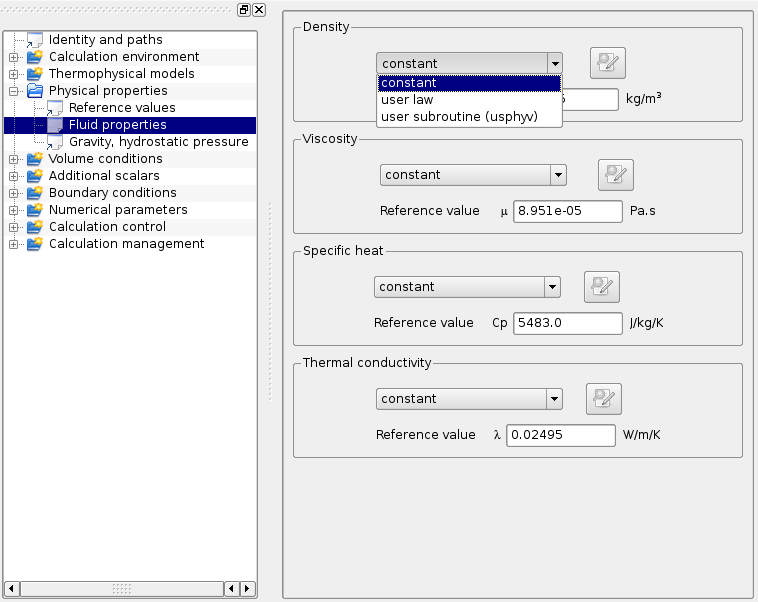
\includegraphics[width=9cm]{V-60} \\
\\
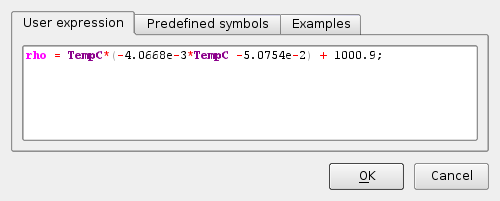
\includegraphics[width=9cm]{V-60bis}
\end{tabular}
\caption{Fluid properties - Variable density}
\label{fig1_e3}
\end{center}
\end{figure}

\newpage
As the density is variable, the influence of gravity has to be considered. In the
heading {\itshape Physical properties} go to
{\itshape Gravity, hydrostatic pressure} and set the value of each component of
the gravity vector.

\begin{figure}[h!]
\begin{center}
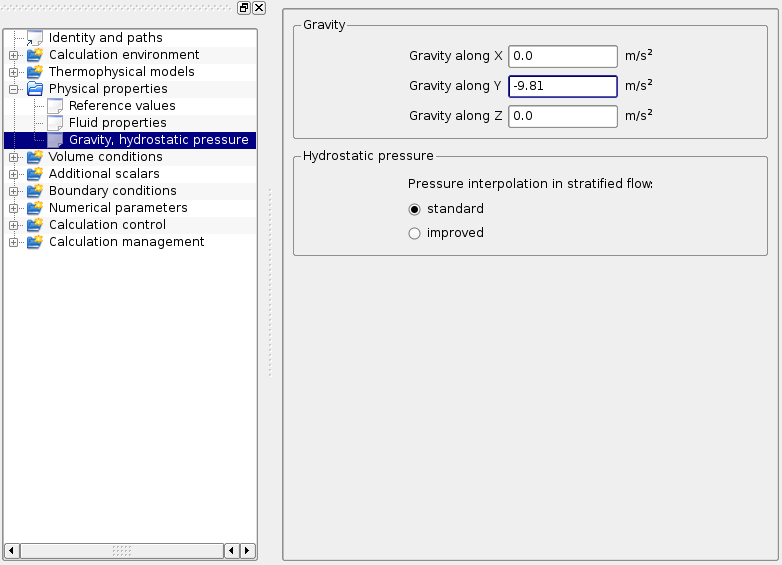
\includegraphics[width=12cm]{V-61}
\caption{Fluid properties - Gravity}
\label{fig2_e3}
\end{center}
\end{figure}


\newpage
Add a monitoring point close to the entry boundary condition in the
{\itshape Output control} item.

\begin{center}
\begin{tabular}{|c|c|c|c|}
\hline
Points & X(m) & Y(m) & Z(m)\\
\hline
9 & -0.5 & 2.25 & 0 \\
\hline
\end{tabular}
\end{center}

\begin{figure}[h!]
\begin{center}
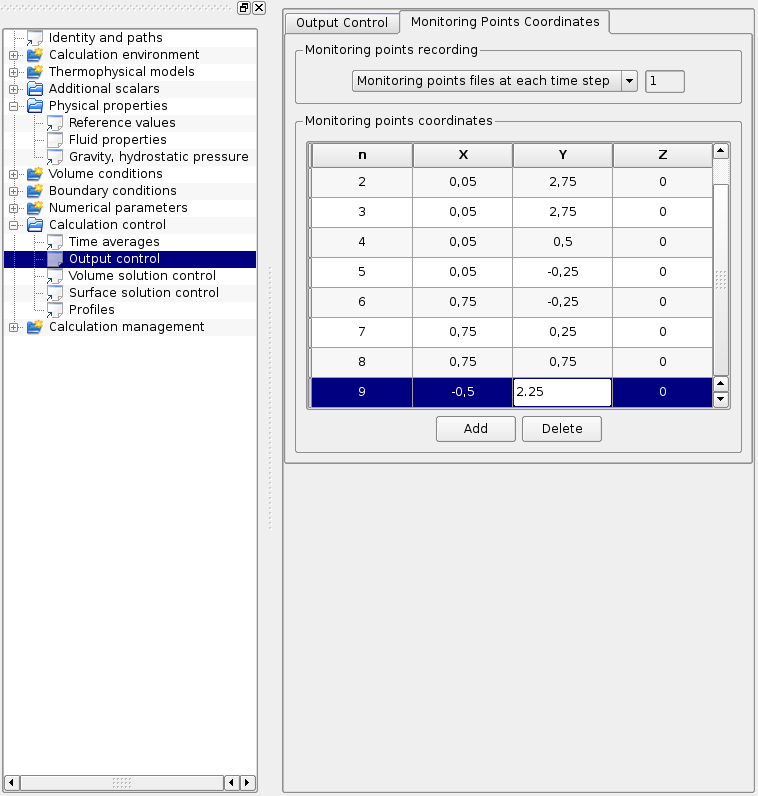
\includegraphics[width=12cm]{V-62}
\caption{New monitoring probe}
\label{fig3_e3}
\end{center}
\end{figure}


\newpage
After completing the interface, before running the calculation,
some Fortran user routines need to be modified.

Go to the folder SRC/REFERENCE/base and copy {\itshape usclim.f90} in the SRC directory.

\textbf{usclim.f90}\\
In this case, {\itshape usclim.f90} is used to specify the time dependent boundary
condition for
the temperature. Refer to the comments in the routine or to the \CS user manual
for more information on this routine.\\
In our case, you need to identify the boundary faces of color 1. The command\\
\texttt{call getfbr('1',nlelt,lstelt)}
will return an integer \texttt{nlelt}, corresponding to the number of boundary faces of
color 1, and an integer array \texttt{lstelt} containing the list of the \texttt{nlelt} boundary
faces of color 1. Note that the string '1' can be more complex and combine
different colors, group references or geometrical criteria, with the same syntax
as in the Graphical Interface.

For each boundary face \texttt{ifac} in the list, the Dirichlet value is given in the
multi-dimension array \texttt{rcodcl} as follows:
\begin{verbatim}
if (ttcabs.lt.3.8d0) then
  do ielt = 1, nlelt
    ifac = lstelt(ielt)
    rcodcl(ifac,isca(1),1) = 20.d0 + 100.d0*ttcabs
  enddo
else
  do ielt = 1, nlelt
    ifac = lstelt(ielt)
    rcodcl(ifac,isca(1),1) = 400.d0
  enddo
endif
\end{verbatim}
\texttt{isca(1)} refers to the first scalar and \texttt{ttcabs} is the current physical time.

See the example file in the directory \texttt{examples} for the complete
{\itshape usclim.f90} file.

Note that, although the inlet boundary conditions for temperature are specified
in the {\itshape usclim.f90} file, it is necessary to specify them also in the
Graphical Interface. The value given in the Interface can be anything, it will
be overwritten by the Fortran routine.

After updating the Fortran file, run the calculation as explained in case
2.


\newpage
When a calculation is finished, \CS stores all the necessary elements to
continue the computation in another execution, with total continuity. These
elements are stored in several files, grouped in a RESTART.xxxxxxxx directory, in
the RESU directory.

In this case, after the first calculation is finished, a second calculation will
be run, starting from the results of the first one.


Go directly on the item {\itshape Start/Restart} under the heading
{\itshape Calculation management}.  Activate the {\itshape Calculation restart}
by ticking the ``on'' box. Then click on the folder icon next to it to specify
the restart files to use.

\begin{figure}[h!]
\begin{center}
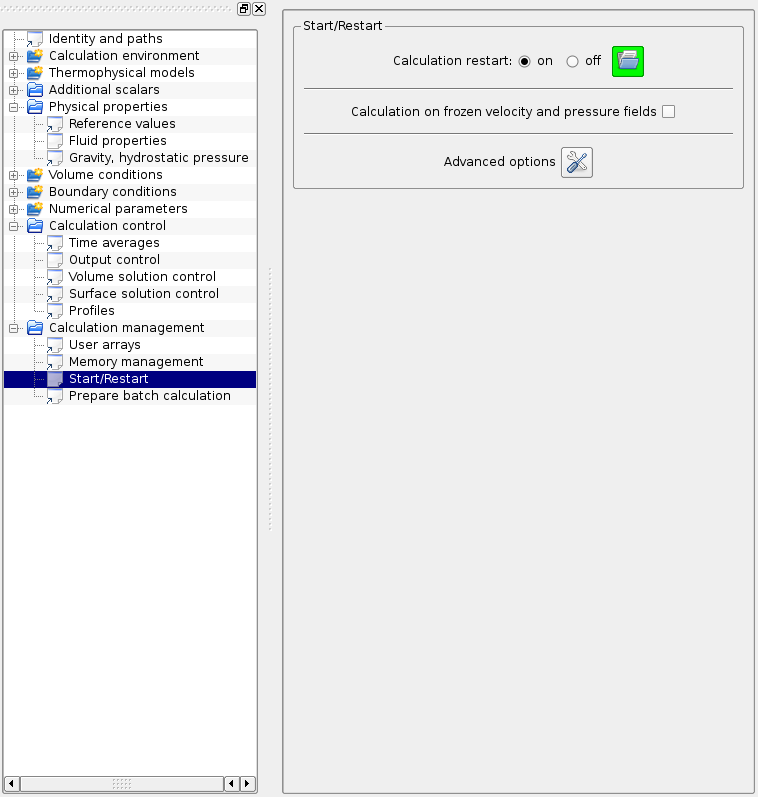
\includegraphics[width=12cm]{V-63}
\caption{Start / Restart}
\label{fig4_e3}
\end{center}
\end{figure}


\newpage
A window opens, with the architecture of the study sub-directories. Open the
RESU folder and click on the folder RESTART.xxxxxxxx (where xxxxxxxx corresponds
to the reference of the first calculation). Then click on {\itshape Validate}.

\begin{figure}[h!]
\begin{center}
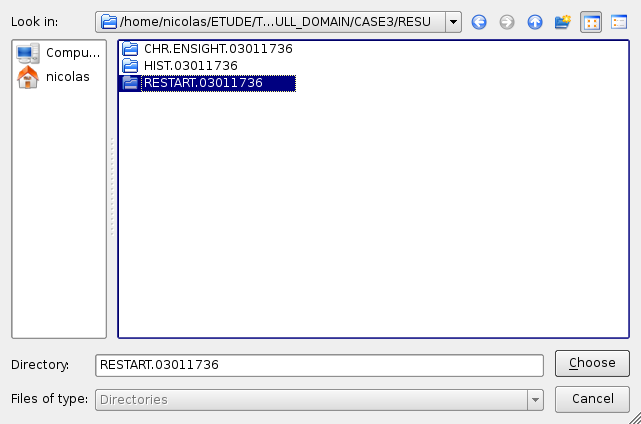
\includegraphics[width=10cm]{V-64}
\caption{Start / Restart - Selection of the restart directory}
\label{fig5_e3}
\end{center}
\end{figure}


\newpage
Go to the {\itshape Time step} item under the heading {\itshape Numerical parameters} and change the number of iterations. It must be the total number of
iterations, from the beginning of the first calculation.\\

The first calculation was done with 300 iterations and another 400 iterations
are needed for the present case. Therefore the value 700 must be entered.

\begin{figure}[h!]
\begin{center}
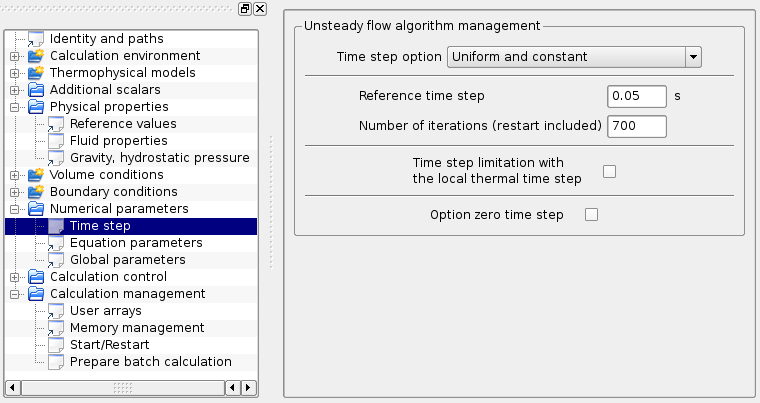
\includegraphics[width=12cm]{V-65}
\caption{Time step}
\label{fig6_e3}
\end{center}
\end{figure}

Eventually, run the calculation.
